%{{第六十五回}}{第六十五回}}

\chapter{贾二舍偷娶尤二姨 尤三姐思嫁柳二郎}
{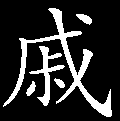
\includegraphics[width=3mm]{../Images/00005}\kaishu 笔笔叙二姐温柔和顺,高凤姐十倍,言语行事,胜凤姐五分,堪为贾琏二房,所以深着凤姐不念宗祠血食,为贾宅第一罪人。纲目书法!}

{\kaishu 文有双管齐下法,此文是也。事在宁府,却把凤姐之奸毅刻薄、平儿之任侠直鲠、李纨之号菩萨、探春之号玫瑰、林姑娘之怕倒、薛姑娘之怕化,一时齐现,是何等妙文!}

话说贾琏、贾珍、贾蓉等三人商议,事事妥贴,至初二日,先将尤老和三姐送入新房。尤老一看,虽不似贾蓉口内之言,也十分齐备,母女二人已称了心。\elegantpar{鲍二夫妇}{鲍二家的换人了}见了如一盆火,赶着尤老一口一声唤老娘,又或是老太太;赶着三姐唤三姨,或是姨娘。至次日五更天,一乘素轿,将二姐抬来。各色香烛纸马,并铺盖以及酒饭,早已备得十分妥当。一时,贾琏素服坐了小轿而来,拜过天地,焚了纸马。那尤老见二姐身上头上焕然一新,不似在家模样,十分得意。搀入洞房。是夜贾琏同他颠鸾倒凤,百般恩爱,不消细说。

那贾琏越看越爱,越瞧越喜,不知怎生奉承这二姐,乃命鲍二等人不许提三说二的,直以奶奶称之,自己也称奶奶,竟将凤姐一笔勾倒。有时回家中,只说在东府有事羁绊,凤姐辈因知他和贾珍相得,自然是或有事商议,也不疑心。再家下人虽多,都不管这些事。便有那游手好闲专打听小事的人,也都去奉承贾琏,乘机讨些便宜,谁肯去露风。于是贾琏深感贾珍不尽。贾琏一月出五两银子做天天的供给。若不来时,他母女三人一处吃饭;若贾琏来了,他夫妻二人一处吃,他母女便回房自吃。贾琏又将自己积年所有的梯己,一并搬了与二姐收着,又将凤姐素日之为人行事,\elegantpar{枕边衾内尽情告诉了他,只等一死,便接他进去}{鲍二家的过错哪有这国舅重,可惜}。二姐听了,自是愿意。当下十来个人,倒也过起日子来,十分丰足。

眼见已是两个月光景。这日贾珍在铁槛寺作完佛事,晚间回家时,因与他姨妹久别,\elegantpar{竟要去探望探望}{有何可探望}。先命小厮去打听贾琏在与不在,小厮回来说不在。贾珍欢喜,将左右一概先遣回去,只留两个心腹小童牵马。一时,到了新房,已是掌灯时分,悄悄入去。两个小厮将马拴在圈内,自往下房去听候。

贾珍进来,屋内才点灯,先看过了尤氏母女,然后二姐出见,贾珍仍唤二姨。大家吃茶,说了一回闲话。贾珍因笑说:``我作的这保山如何?若错过了,打着灯笼还没处寻,过日你姐姐还备了礼来瞧你们呢。''说话之间,尤二姐已命人预备下酒馔,关起门来,都是一家人,原无避讳。那鲍二来请安,贾珍便说:``你还是个有良心的小子,所以叫你来伏侍。日后自有大用你之处,不可在外头吃酒生事。我自然赏你。倘或这里短了什么,你琏二爷事多,那里人杂,你只管去回我。\elegantpar{我们弟兄不比别人}{是是是,你们好兄弟}。''鲍二答应道:``是,小的知道。若小的不尽心,除非不要这脑袋了。''贾珍点头说:``要你知道。''当下四人一处吃酒。尤二姐知局,便邀他母亲说:``我怪怕的,妈同我到那边走走来。''尤老也会意,便真个同他出来,只剩小丫头们。贾珍便和三姐挨肩擦脸,百般轻薄起来。小丫头子们看不过,也都躲了出去,凭他两个自在取乐,不知作些什么勾当。

跟的两个小厮都在厨下和鲍二饮酒,鲍二女人上灶。忽见两个丫头也走了来嘲笑,要吃酒。鲍二因说:``姐儿们不在上头伏侍,也偷来了。一时叫起来没人,又是事。''他女人骂道:``糊涂浑呛了的忘八!你撞丧那黄汤罢。撞丧醉了,夹着你那膫子挺你的尸去。叫不叫,与你屄相干!一应有我承当,风雨横竖洒不着你头上来。''这鲍二{原因妻子发迹的,近日越发亏他}{是头一个妻子,上吊}。自己除赚钱吃酒之外,一概不管,贾琏等也不肯责备他,故他视妻如母,百依百随,且吃够了便去睡觉。这里鲍二家的陪着这些丫鬟小厮吃酒,讨他们的好,准备在贾珍前上好。

四人正吃的高兴,忽听扣门之声,鲍二家的忙出来开门,看见是贾琏下马,问有事无事。鲍二女人便悄悄告他说:``大爷在这里西院里呢。''贾琏听了,便回至卧房。只见尤二姐和他母亲都在房中,见他来了,二人面上便有些讪讪的。贾琏反推不知,只命:``快拿酒来,咱们吃两杯好睡觉。我今日很乏了。''尤二姐忙上来陪笑接衣奉茶,问长问短。贾琏喜的心痒难受。一时鲍二家的端上酒来,二人对饮。他丈母不吃,自回房中睡去了。两个小丫头分了一个过来伏侍。

贾琏的心腹小童隆儿拴马去,见已有了一匹马,细瞧一瞧,知是贾珍的,心下会意,也来厨下。只见喜儿寿儿两个正在那里坐着吃酒,见他来了,也都会意,故笑道:``你这会子来的巧。我们因赶不上爷的马,恐怕犯夜,往这里来借宿一宵的。''隆儿便笑道:``有的是炕,只管睡。我是二爷使我送月银的,交给了奶奶,我也不回去了。''喜儿便说:``我们吃多了,你来吃一钟。''隆儿才坐下,端起杯来,忽听马棚内闹将起来。原来二马同槽,不能相容,互相蹶踢起来。隆儿等慌的忙放下酒杯,出来喝马,好容易喝住,另拴好了,方进来。鲍二家的笑说:``你三人就在这里罢,茶也现成了,我可去了。''说着,带门出去。这里喜儿喝了几杯,已是楞子眼了。隆儿寿儿关了门,回头见喜儿直挺挺的仰卧炕上,二人便推他说:``好兄弟,起来好生睡,只顾你一个人,我们就苦了。''那喜儿便说道:``咱们今儿\elegantpar{可要公公道道的贴一炉子烧饼,要有一个充正经的人}{恐怕不是好话},我痛把你妈一肏。''隆儿寿儿见他醉了,也不必多说,只得吹了灯,将就睡下。

尤二姐听见马闹,心下便不自安,只管用言语混乱贾琏。那贾琏吃了几杯,春兴发作,便命收了酒果,掩门宽衣。尤二姐只穿着大红小袄,散挽乌云,满脸春色,比白日更增了颜色。贾琏搂他笑道:``人人都说我们那夜叉婆齐整,如今我看来,给你拾鞋也不要。''尤二姐道:``我虽标致,却无品行。看来到底是不标致的好。''贾琏忙问道:``这话如何说?我却不解。''尤二姐滴泪说道:``你们拿我作愚人待,什么事我不知。我如今和你作了两个月夫妻,日子虽浅,我也知你不是愚人。我生是你的人,死是你的鬼,如今既作了夫妻,我终身靠你,岂敢瞒藏一字。我算是有靠,将来我妹子却如何结果?据我看来,这个形景恐非长策,要作长久之计方可。''贾琏听了,笑道:``你且放心,我不是拈酸吃醋之辈。前事我已尽知,你也不必惊慌。你因妹夫倒是作兄的,自然不好意思,不如我去破了这例。''说着走了,便至西院中来,只见窗内灯烛辉煌,二人正吃酒取乐。

贾琏便推门进去,笑说:``大爷在这里,兄弟来请安。''贾珍羞的无话,只得起身让坐。贾琏忙笑道:``何必又作如此景象,咱们弟兄从前是如何样来!大哥为我操心,我今日粉身碎骨,感激不尽。大哥若多心,我意何安。从此以后,还求大哥如昔方好;不然,兄弟能可绝后,再不敢到此处来了。''说着,便要跪下。慌的贾珍连忙搀起,只说:``兄弟怎么说,我无不领命。''贾琏忙命人:``看酒来,我和大哥吃两杯。''又拉尤三姐说:``你过来,陪小叔子一杯。''贾珍笑着说:``老二,到底是你,哥哥必要吃干这钟。''说着,一扬脖。

尤三姐站在炕上,指贾琏笑道:``你不用和我花马吊嘴的。`清水下杂面,你吃我看见'\href{../Text/part0069_split_000.html\#lnkback_1_a}{\textsuperscript{①}};`提着影戏人子上场,好歹别戳破这层纸儿'。你别油蒙了心,打量我们不知道你府上的事。这会子花了几个臭钱,你们哥儿俩拿着我们姐儿两个权当粉头来取乐儿,你们就打错了算盘了。我也知道你那老婆太难缠,如今把我姐姐拐了来做二房,`偷的锣儿敲不得'。我也要会会那凤奶奶去,看他是几个脑袋几只手。若大家好取和便罢;倘若有一点叫人过不去,我有本事先把你两个的牛黄狗宝掏了出来,再和那泼妇拼了这命,也不算是尤三姑奶奶!喝酒怕什么,咱们就喝!''说着,自己绰起壶来斟了一杯,自己先喝了半杯,搂过贾琏的脖子来就灌,说:``\elegantpar {我和你哥哥已经吃过了,咱们来亲香亲香。}{三姐前文一直未叙}''唬的贾琏酒都醒了。贾珍也不承望尤三姐这等无耻老辣。弟兄两个本是风月场中耍惯的,不想今日反被这闺女一席话说住。尤三姐一叠声又叫:``将姐姐请来,要乐咱们四个一处同乐。俗语说`便宜不过当家',他们是弟兄,咱们是姊妹,又不是外人,只管上来。''尤二姐反不好意思起来。贾珍得便就要一溜,尤三姐那里肯放。贾珍此时方后悔,不承望他是这种为人,与贾琏反不好轻薄起来。

这尤三姐松松挽着头发,大红袄子半掩半开,露着葱绿抹胸,一痕雪脯。底下绿裤红鞋,\elegantpar{一对金莲或翘或并}{这还少缠了脚的},没半刻斯文。两个坠子却似打秋千一般,灯光之下,越显得柳眉笼翠雾,檀口点丹砂。本是一双秋水眼,再吃了酒,又添了饧涩淫浪,不独将他二姊压倒,据珍琏评去,所见过的上下贵贱若干女子,皆未有此绰约风流者。二人已酥麻如醉,不禁去招他一招,他那淫态风情,反将二人禁住。那尤三姐放出手眼来略试了一试,他弟兄两个竟全然无一点别识别见,连口中一句响亮话都没了,不过是酒色二字而已。自己高谈阔论,任意挥霍洒落一阵,拿他弟兄二人嘲笑取乐,竟真是他嫖了男人,并非男人淫了他。一时他的酒足兴尽,也不容他弟兄多坐,撵了出去,自己关门睡去了。

自此后,或略有丫鬟婆娘不到之处,便将贾琏、贾珍、贾蓉三个泼声厉言痛骂,说他爷儿三个诓骗了他寡妇孤女。贾珍回去之后,以后亦不敢轻易再来。有时尤三姐自己高了兴悄命小厮来请,方敢去一会,到了这里,也只好随他的便。谁知这尤三姐天生脾气不堪,仗着自己风流标致,偏要打扮的出色,另式作出许多万人不及的淫情浪态来,哄的男子们垂涎落魄,欲近不能,欲远不舍,迷离颠倒,他以为乐。他母姊二人也十分相劝,他反说:``姐姐糊涂。咱们金玉一般的人,白叫这两个现世宝沾污了去,也算无能。而且他家有一个极利害的女人,如今瞒着他不知,咱们方安。倘或一日他知道了,岂有干休之理,势必有一场大闹,不知谁生谁死。趁如今我不拿他们取乐作践准折,到那时白落个臭名,后悔不及。''因此一说,他母女见不听劝,也只得罢了。那尤三姐天天挑拣穿吃,打了银的,又要金的;有了珠子,又要宝石;吃的肥鹅,又宰肥鸭。或不趁心,连桌一推;衣裳不如意,不论绫缎新整,便用剪刀剪碎,撕一条,骂一句。究竟贾珍等何曾随意了一日,反花了许多昧心钱。

贾琏来了,只在二姐房内,心中也悔上来。无奈二姐倒是个多情人,以为贾琏是终身之主了,凡事倒还知疼着痒。若论起温柔和顺,凡事必商必议,不敢恃才自专,实较凤姐高十倍;若论标致,言谈行事,也胜五分。虽然如今改过,但已经失了脚,有了一个``淫''字,凭他有甚好处也不算了。偏这贾琏又说:``谁人无错,知过必改就好。''故不提已往之淫,只取现今之善,便如胶授漆,似水如鱼,一心一计,誓同生死,那里还有凤平二人在意了?二姐在枕边衾内,也常劝贾琏说:``你和珍大哥商议商议,拣个相熟的人,把三丫头聘了罢。留着他不是常法子,终久要生出事来,怎么处?''贾琏道:``前日我曾回过大哥的,他只是舍不得。我说`是块肥羊肉,只是烫的慌;玫瑰花儿可爱,刺大扎手。咱们未必降的住,正经拣个人聘了罢。'他只意意思思,就丢开手了。你叫我有何法。''二姐道:``你放心。咱们明日先劝三丫头,他肯了,让他自己闹去。闹的无法,少不得聘他。''贾琏听了说:``这话极是。''

至次日,二姐另备了酒,贾琏也不出门,至午间特请他小妹过来,与他母亲上坐。尤三姐便知其意,{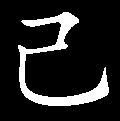
\includegraphics[width=3mm]{../Images/00003}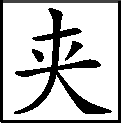
\includegraphics[width=3mm]{../Images/00012}\footnotesize \kaishu 全用醍醐灌顶,全是大翻身大解悟法。}酒过三巡,不用姐姐开口,先便滴泪泣道:{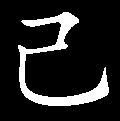
\includegraphics[width=3mm]{../Images/00003}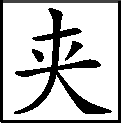
\includegraphics[width=3mm]{../Images/00012}\footnotesize \kaishu 全用如是等语,一洗孽障。}``姐姐今日请我,自有一番大礼要说。但妹子不是那愚人,也不用絮絮叨叨提那从前丑事,我已尽知,说也无益。既如今姐姐也得了好处安身,妈也有了安身之处,我也要自寻归结去,方是正理。但终身大事,一生至一死,非同儿戏。\elegantpar {我如今改过守分,只要我拣一个素日可心如意的人方跟他去。若凭你们拣择,虽是富比石崇,才过子建,貌比潘安的,我心里进不去,也白过了一世。}{传说中的找个老实人嫁了}''贾琏笑道:``这也容易。凭你说是谁就是谁,一应彩礼都有我们置办,母亲也不用操心。''尤三姐泣道:``姐姐知道,不用我说。''贾琏笑问二姐是谁,二姐一时也想不起来。大家想来,贾琏便料定是此人无移了,便拍手笑道:``我知道了。这人原不差,果然好眼力。''二姐笑问是谁,贾琏笑道:``别人他如何进得去,一定是宝玉。''二姐与尤老听了,亦以为然。尤三姐便啐了一口,道:{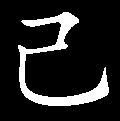
\includegraphics[width=3mm]{../Images/00003}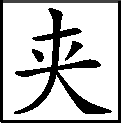
\includegraphics[width=3mm]{../Images/00012}\footnotesize \kaishu 奇,不知何为。}``我们有姊妹十个,也嫁你弟兄十个不成?{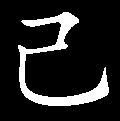
\includegraphics[width=3mm]{../Images/00003}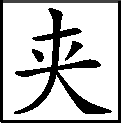
\includegraphics[width=3mm]{../Images/00012}\footnotesize \kaishu 有理之极!}\elegantpar{难道除了你家,天下就没了好男子了不成!}{只从眼前想,五年前?}''{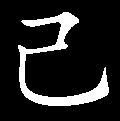
\includegraphics[width=3mm]{../Images/00003}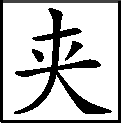
\includegraphics[width=3mm]{../Images/00012}\footnotesize \kaishu 一骂反有理。}众人听了都诧异:``除去他,还有那一个?''{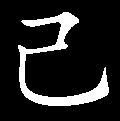
\includegraphics[width=3mm]{../Images/00003}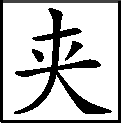
\includegraphics[width=3mm]{../Images/00012}\footnotesize \kaishu 余亦如此想。}尤三姐笑道:``别只在眼前想,姐姐只在五年前想就是了。''{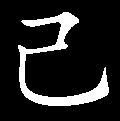
\includegraphics[width=3mm]{../Images/00003}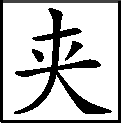
\includegraphics[width=3mm]{../Images/00012}\footnotesize \kaishu 奇甚!}

正说着,忽见贾琏的心腹小厮兴儿走来请贾琏说:``老爷那边紧等着叫爷呢。小的答应往舅老爷那边去了,小的连忙来请。''贾琏又忙问:``昨日家里没人问?''兴儿道:``小的回奶奶说,爷在家庙里同珍大爷商议作百日的事,只怕不能来家。''贾琏忙命拉马,隆儿跟随去了,留下兴儿答应人来事务。

尤二姐拿了两碟菜,命拿大杯斟了酒,就命兴儿在炕沿下蹲着吃,一长一短向他说话儿。问他家里奶奶多大年纪,怎个利害的样子,老太太多大年纪,太太多大年纪,姑娘几个,各样家常等语。兴儿笑嘻嘻的在炕沿下一头吃,一头将荣府之事备细告诉他母女。又说:``我是二门上该班的人。我们共是两班,一班四个,共是八个。这八个人有几个是奶奶的心腹,有几个是爷的心腹。奶奶的心腹我们不敢惹,爷的心腹奶奶的就敢惹。提起我们奶奶来,心里歹毒,口里尖快。我们二爷也算是个好的,那里见得他。倒是跟前的平姑娘为人很好,虽然和奶奶一气,\elegantpar {他倒背着奶奶常作些个好事}{这不是任盈盈?}。小的们凡有了不是,奶奶是容不过的,只求求他去就完了。如今合家大小除了老太太、太太两个人,没有不恨他的,只不过面子情儿怕他。皆因他一时看的人都不及他,只一味哄着老太太、太太两个人喜欢。他说一是一,说二是二,没人敢拦他。又恨不得把银子钱省下来堆成山,好叫老太太、太太说他会过日子,殊不知苦了下人,他讨好儿。估着有好事,他就不等别人去说,他先抓尖儿;或有了不好事或他自己错了,他便一缩头推到别人身上来,他还在旁边拨火儿。如今连他正经婆婆大太太都嫌了他,说他`雀儿拣着旺处飞,黑母鸡一窝儿,自家的事不管,倒替人家去瞎张罗'。若不是老太太在头里,早叫过他去了。''

尤二姐笑道:``你背着他这等说他,将来你又不知怎么说我呢。我又差他一层儿,越发有的说了。''兴儿忙跪下说道:``奶奶要这样说,小的不怕雷打!但凡小的们有造化起来,先娶奶奶时若得了奶奶这样的人,小的们也少挨些打骂,也少提心吊胆的。如今跟爷的这几个人,谁不背前背后称扬奶奶圣德怜下。我们商量着叫二爷要出来,情愿来答应奶奶呢。''尤二姐笑道:``猴儿肏的,还不起来呢。说句顽话,就唬的那样起来。你们作什么来,我还要找了你奶奶去呢。''

兴儿连忙摇手说:``奶奶千万不要去。我告诉奶奶,一辈子别见他才好。嘴甜心苦,两面三刀;上头一脸笑,脚下使绊子;明是一盆火,暗是一把刀:都占全了。只怕三姨的这张嘴还说他不过。奶奶这样斯文良善人,那里是他的对手!''尤氏笑道:``我只以礼待他,他敢怎么样!''兴儿道:``不是小的吃了酒放肆胡说,奶奶便有礼让,他看见奶奶比他标致,又比他得人心,他怎肯干休善罢?人家是醋罐子,他是醋缸醋瓮。凡丫头们二爷多看一眼,他有本事当着爷打个烂羊头。虽然平姑娘在屋里,大约一年二年之间两个有一次到一处,他还要口里掂十个过子呢,气的平姑娘性子发了,哭闹一阵,说:`又不是我自己寻来的,你又浪着劝我,我原不依,你反说我反了,这会子又这样。'他一般的也罢了,倒央告平姑娘。''尤二姐笑道:``可是扯谎?这样一个夜叉,怎么反怕屋里的人呢?''兴儿道:``这就是俗语说的`天下逃不过一个理字去'了。这平儿是他自幼的丫头,陪了过来一共四个,嫁人的嫁人,死的死了,只剩了这个心腹。他原为收了屋里,一则显他贤良名儿,二则又叫拴爷的心,好不外头走邪的。又还有一段因果:\elegantpar {我们家的规矩,凡爷们大了,未娶亲之先都先放两个人伏侍的。}{算来宝玉就是袭人和晴雯了}二爷原有两个,谁知他来了没半年,都寻出不是来,都打发出去了。别人虽不好说,自己脸上过不去,所以强逼着平姑娘作了房里人。那平姑娘又是个正经人,从不把这一件事放在心上,也不会挑妻窝夫的,倒一味忠心赤胆伏侍他,才容下了。''

尤二姐笑道:``原来如此。但我听见你们家还有一位寡妇奶奶和几位姑娘。他这样利害,这些人如何依得?''兴儿拍手笑道:``原来奶奶不知道。我们家这位寡妇奶奶,他的浑名叫作`大菩萨',第一个善德人。我们家的规矩又大,寡妇奶奶们不管事,只宜清净守节。妙在姑娘又多,只把姑娘们交给他,看书写字,学针线,学道理,这是他的责任。除此问事不知,说事不管。只因这一向他病了,事多,这大奶奶暂管几日。究竟也无可管,不过是按例而行,不像他多事逞才。我们大姑娘不用说,但凡不好也没这段大福了。二姑娘的浑名是`二木头',戳一针也不知`嗳哟'一声。三姑娘的浑名是`玫瑰花'。''尤氏姊妹忙笑问何意。兴儿笑道:``玫瑰花又红又香,无人不爱的,只是刺戳手。也是一位神道,可惜不是太太养的,`老鸹窝里出凤凰'。四姑娘小,他正经是珍大爷亲妹子,因自幼无母,老太太命太太抱过来养这么大,也是一位不管事的。奶奶不知道,我们家的姑娘不算,另外有两个姑娘,真是天上少有,地下无双。一个是咱们姑太太的女儿,姓林,小名儿叫什么黛玉,面庞身段和三姨不差什么,一肚子文章,只是一身多病,这样的天,还穿夹的,出来风儿一吹就倒了。我们这起没王法的嘴都悄悄的叫他`多病西施'。还有一位姨太太的女儿,姓薛,叫什么宝钗,竟是雪堆出来的。每常出门或上车,或一时院子里瞥见一眼,我们鬼使神差,见了他两个,不敢出气儿。''尤二姐笑道:``你们大家规矩,虽然你们小孩子进的去,然遇见小姐们,原该远远藏开。''兴儿摇手道:``不是,不是。那正经大礼,自然远远的藏开,自不必说。就藏开了,\elegantpar {自己不敢出气,是生怕这气大了,吹倒了姓林的;气暖了,吹化了姓薛的。}{奇甚!}''说的满屋里都笑起来了。要知端的,下回分解。

{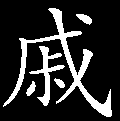
\includegraphics[width=3mm]{../Images/00005}\kaishu        总评:房内兄弟聚}麀{,棚内两马相闹;小厮与家母饮酒,小姨与姐夫同床。可见有是主必有是奴,有是兄必有是弟,有是姐必有是妹,有是人必有是马。}

% {\href{../Text/part0069_split_000.html\#navto_1_a}{①}
% ``清水下杂面,你吃我看见'':或谓``见''字应归下句,这个歇后语只作``清水下杂面,你吃我看'',但第七十一回这句俗语再次出现时,作``清水下杂面,你吃我也见''。}
